\documentclass[12pt,a4paper]{article}
\usepackage[margin=0.5in]{geometry} % custom margins
\usepackage{graphicx}
\graphicspath{ {./Images/} }
\usepackage{array,mathtools}
\usepackage{listings}

% When writing indented paragraphs:
% \usepackage{indentfirst}

% To supress page numbers:
% \usepackage{nopageno}

\begin{document}
\begin{center}
    
\includegraphics[width=\textwidth]{./Images/Header.jpeg}
    \vfill
    \textbf{\Large{Report for Experiment \#3\\
    Arithmetic and Logic Unit}}
    \vfill
    Trevor Smith\\
    February 25, 2022
    \vfill
\end{center}

\newpage

\section*{Prelab:}

Below is a table of test vectors used to verify the code.

$\setlength{\arraycolsep}{20pt}
\begin{array}[R]{r|r|r|r|r|r}
	a & b & sel & f & ovf & take\_branch \\ \hline
	0000\ 0000 & 0000\ 0000 & 000 & 0000\ 0000 & 0 & 0 \\
	0011\ 1111 & 0011\ 1111 & 000 & 0111\ 1110 & 0 & 0 \\
	0011\ 1111 & 0011\ 1111 & 001 & 1100\ 0000 & 0 & 0 \\
	0011\ 1111 & 0011\ 1111 & 010 & 0011\ 1111 & 0 & 0 \\
	0011\ 1111 & 0011\ 1111 & 011 & 0011\ 1111 & 0 & 0 \\
	0111\ 1100 & 0011\ 1111 & 000 & 1011\ 1011 & 1 & 0 \\
	0111\ 1111 & 0000\ 0010 & 100 & 0011\ 1111 & 0 & 0 \\
	0111\ 1111 & 0000\ 0010 & 101 & 1111\ 1100 & 0 & 0 \\
	0111\ 1111 & 0000\ 0010 & 110 & 0000\ 0000 & 0 & 0 \\
	0111\ 1111 & 0000\ 0010 & 111 & 0000\ 0000 & 0 & 1 \\
	0111\ 1111 & 0111\ 1111 & 111 & 0000\ 0000 & 0 & 0 \\
	0111\ 1111 & 0111\ 1111 & 110 & 0000\ 0000 & 0 & 1 \\
	1000\ 0001 & 0000\ 0010 & 100 & 1100\ 0000 & 0 & 0 \\
\end{array}$ \\ \\

The code itself, along with an image of the test bench output,
can be found in the appendix.

\section*{Results and Analysis:}

The eight-bit partial ALU from the previous lab was built on, completing
the full Arithmetic Logic Unit (ALU). This was achieved primarily by extending
the `case' control structure used in the partial ALU, which picks an
operation depending on the value of `sel'. \\

The program was then streamed to a PYNQ board. A discrepancy was found
between the ALU module and the provided top-level in the naming of `sel'.
This was fixed and the program worked as expected. \\

Because the number of switches on the PYNQ board are not sufficient
for this full ALU, `Virtual Inputs' were used to test the board in real-time.
This was found to be effective, and much more straightforward/easy to follow
than using a bunch of buttons and switches scattered all over the place.


\section*{Conclusion and Recommendations:}

An ALU with an eight-bit adder, bitwise OR and AND, left/right bit shifter,
and brancher was successfully implemented and tested. 
At this point there is much more familiarity with the Vivado software
and the verilog control structures/syntax. That said, very little was
actually added to the previous lab's implementation, which did not do 
much to push the lab worker's current limits.

\newpage
\section*{Appendices:}

\subsection{Appendix A: Design Program Files}

\begin{lstlisting}

module eightbit_alu(
    input signed [7:0]a,
    input signed [7:0]b,
    input [2:0]sel,
    output signed [7:0]f,
    output ovf,
    output take_branch
);

    reg [7:0]f;
    reg ovf;
    reg take_branch;

    always @(a or b or sel) begin
    case (sel)

        3'b000:  // addition
            begin 
                f = a + b;
                ovf = f[7]? ~(a[7] | b[7]):a[7] & b[7];
                take_branch = 0;
            end
        3'b001:  // inversion
            begin
                f = ~b;
                ovf = 0;
                take_branch = 0;
            end
        3'b010:  // bitwise AND
            begin
                f = a & b;
                ovf = 0;
                take_branch = 0;
            end
        3'b011:  // bitwise OR
            begin
                f = a | b;
                ovf = 0;
                take_branch = 0;
            end
        3'b100:  // arithmetic shift right
            begin
                f = a >>> 1;
                ovf = 0;
                take_branch = 0;
            end
        3'b101:  // logical shift left
            begin
                f = a << b;
                ovf = 0;
                take_branch = 0;
            end
        3'b110:  // branch if equal
            begin
                take_branch = a == b;
                ovf = 0;
                f = 0;
            end
        3'b111:  // branch if inequal
            begin
                take_branch = a != b;
                ovf = 0;
                f = 0;
            end

    endcase
end

endmodule


module eightbit_alu_tb();

    reg [7:0]a;
    reg [7:0]b;
    reg [2:0]sel;
    wire [7:0]f;
    wire ovf;
    wire take_branch;

    eightbit_alu uut(
        .a(a),
        .b(b),
        .sel(sel),
        .f(f),
        .ovf(ovf),
        .take_branch(take_branch)
    );

    initial
    begin
        a = 0;
        b = 0;
        sel = 0;

        #100;

        a = 63;
        b = 63;

        #100;

        sel = 1;

        #100;

        sel = 2;

        #100;

        sel = 3;

        #100;

        sel = 0;
        a = 124;

        #100;

        b = 124;

        #100;

        a = 127;
        b = 2;
        sel = 4;

        #100;

        sel = 5;

        #100;

        sel = 6;

        #100;

        sel = 7;

        #100;

        b = 127;

        #100;

        sel = 6;

        #100;

        a = -127;
        sel = 4;

    end


endmodule

\end{lstlisting}

\subsection{Appendix B: Output Screen Capture}

\begin{figure}[h]
	\centering
	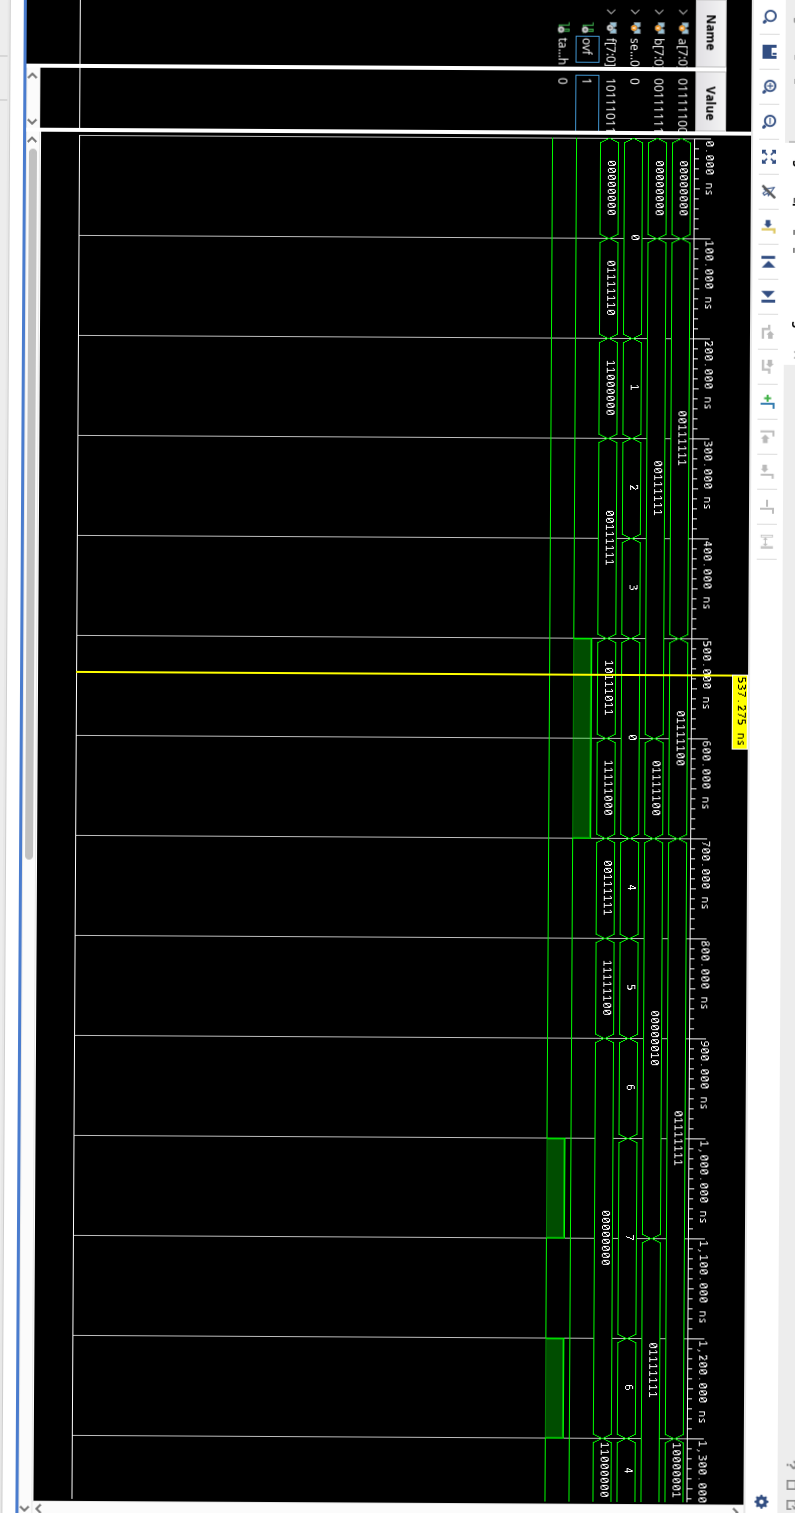
\includegraphics[width=\linewidth]{image}
	\caption{Test bench output}
\end{figure}

\end{document}
